\documentclass{subfiles}
\begin{document}
\begin{figure}[h!]
    \begin{subfigure}[b]{0.5\textwidth}
        \centering
        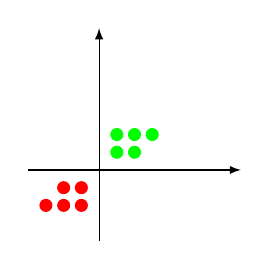
\begin{tikzpicture}[every node/.style={scale = 0.5}, scale = 0.45]

            \draw[-latex] (-2, 0) -- (4, 0);
            \draw[-latex] (0, -2) -- (0, 4);

            \node (r1) at (-0.5, -0.5) [circle, fill = red] {};
            \node (r2) at (-1, -0.5) [circle, fill = red] {};
            \node (r3) at (-0.5, -1) [circle, fill = red] {};
            \node (r4) at (-1, -1) [circle, fill = red] {};
            \node (r5) at (-1.5, -1) [circle, fill = red] {};

            \node (g1) at (0.5, 0.5) [circle, fill = green] {};
            \node (g2) at (1, 0.5) [circle, fill = green] {};
            \node (g3) at (0.5, 1) [circle, fill = green] {};
            \node (g4) at (1, 1) [circle, fill = green] {};
            \node (g5) at (1.5, 1) [circle, fill = green] {};
        \end{tikzpicture}
        \subcaption{Dati base}
        \label{Fig:1.a}
    \end{subfigure}
    \begin{subfigure}[b]{0.5\textwidth}
        \centering
        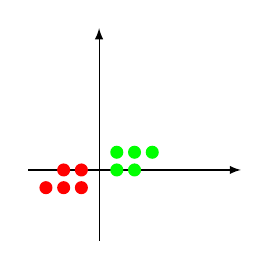
\begin{tikzpicture}[every node/.style={scale = 0.5}, scale = 0.45]

            \draw[-latex] (-2, 0) -- (4, 0);
            \draw[-latex] (0, -2) -- (0, 4);

            \node (r1) at (-0.5, 0) [circle, fill = red] {};
            \node (r2) at (-1, 0) [circle, fill = red] {};
            \node (r3) at (-0.5, -0.5) [circle, fill = red] {};
            \node (r4) at (-1, -0.5) [circle, fill = red] {};
            \node (r5) at (-1.5, -0.5) [circle, fill = red] {};

            \node (g1) at (0.5, 0) [circle, fill = green] {};
            \node (g2) at (1, 0) [circle, fill = green] {};
            \node (g3) at (0.5, 0.5) [circle, fill = green] {};
            \node (g4) at (1, 0.5) [circle, fill = green] {};
            \node (g5) at (1.5, 0.5) [circle, fill = green] {};
        \end{tikzpicture}
        \subcaption{Dati riferiti agli autovalori}
        \label{Fig:1.b}
    \end{subfigure}
\end{figure}
\end{document}